\chapter{Results and Discussion}\label{C:results}\label{C:evaluation}

For our tool is be useful, it has to achieve the goal of identifying redundant test cases. To evaluate this goal, we need to execute and analyse experiments. The key idea of the chapter is to discuss our approach to the experiments and discuss the results. The chapter starts by discussing the method we used to perform several experiments with. It then discusses the benchmarks used to execute these experiments on. After this, the remainder of the chapter reports on the outcome of the experiments. These experiments explore the use of our tool on a realistic benchmark suite and the important factors of interest are: the time taken, number of comparisons, the types of redundant tests identified and the overall cost of performance (time) vs precision (number and types of tests identified).

There are two points that the reader needs to be aware of. Firstly, in the tables below, a `+' represents a significant increase, `-' a significant decrease and `=' represents no significant difference. Secondly, the graphs are displayed using a logarithm scale.

\section{Experimental Method}

The experimental method is key to producing believable and reproducible results. The next three sections discuss the process of our experiments. Before we could conduct the experiments, the benchmarks had to have their test suites traced. This involved setting the benchmarks up locally and then tracing the tests with the AspectJ class loader on a local machine. The trace information was then used in several experiments. The experiments consisted of using the tool with the different techniques discussed in Chapter \ref{C:workdone}, each being executed 30 times per benchmark. The experiments explored the following: Pipeline length, K depth, Parameters and Weighting. We solved the issue of running a large number of tests by using a grid computing system. After the results had been gathered, we used a Wilcoxon signed rank test \cite{wilcoxon1945individual} to determine whether the results were significantly different or not. The significance level used was 95\% with a null hypothesis of the two samples median being equal. Overall, seven different settings were run per benchmark with each setting being run 30 times. For every setting experimented on, they all consisted of a first pipeline stage using a ``unique method calls" spectrum filter. 

\section{Environmental Methodologies}
\label{enviro}
As discussed in Section \ref{performanceEvalBG} there are a variety of challenges that present themselves when using Java to evaluate performance. The following section discusses these challenges.

\subsection{Grid Computing}
The experiments were executed on a grid computing system, with a total of 150 jobs queued on the grid at a single time. When using a grid system it is important to ensure that all the machines used are the same for every experiment. The grid system allowed for particular types of machines to be specified -- 8GB DDR3 RAM, Linux 4.0.5 64 bit system and an Intel Core i7-3770 CPU running @ 3.40GHz.

\subsection{Measuring Time }
The time taken is an important variable in evaluating the performance of a tool. The tool uses the notation of CPU time to measure the time taken. The CPU time is the measure of time in nanoseconds that the tool spent on the CPU. A concern is if a user logs in during analysis, the grid system pauses the tool and the machine may move the program into virtual memory on disk. This is dependent on the amount of resources that the user needs. When the user logs out, the grid system will unpause the tool. The occurrence of pausing and unpausing may cause non-deterministic behaviour.  We limited the issues by running the tests overnight when users were unlikely to log in.

We had to decide what we should measure in regard to the time taken. Ideally, we would measure the start up cost of the tool as well as the time taken to analyse the trace information. The start up of the tool involved loading the trace information into memory. The issue was when a large number of instances of the tool were running concurrently on the grid. These instances were attempting to access the same trace information file stored on the network. The stress on the network introduces a large amount of non-deterministic behaviour. Therefore, the tool disregards the start up time when measuring the total time taken.

\subsubsection{Heap Size}
The heap is the location that the JVM uses to store objects that the  application executed creates. The amount of heap that was allocated to the JVM was 6GB for every benchmark on every run.

\subsection{Software Environment}

We used a concurrent-mark-sweep garbage collection strategy (default). This approach uses multiple threads to scan the heap, mark unused objects and recycle them \cite{oracle2015}. It allows for a high throughput however, tends to use more CPU time than other strategies. This was deemed worth the trade off as memory was the bottleneck rather than the CPU.

\section{Benchmarks}
\label{S:bench}
The benchmarks had to be realistic real world projects otherwise the experiments would lose credibility. They were located by looking at popular Java frameworks, Github repositories and David Pearce's personal projects. For us to consider a benchmark, it had to be Java based, have a reasonable number of tests (40+) and be open source. The benchmarks that used either Ant or Gradle build tools were favoured due to their easier build process.

A variety of test types and sizes of benchmarks were used to fully evaluate the tool. Tables \ref{large_testdes} , \ref{small_testdes}, \ref{large_test} and \ref{small_test} show information on the benchmarks. The information shown is a description of each benchmark, the authors, types of tests, number of tests traced, lines of code and version used. An important thing to note is that the number of tests is only the amount that were traced. We choose a range of test types, David J Pearce's projects contain end to end tests which run through a whole module at once. The other benchmarks test units of code at a time. Having a range of test types and sizes gives a wider evaluation view and insight into the potential situations where different settings may not be helpful in achieving the aim.

Some of the benchmarks produced up to 100,000 method calls per test, each with parameter information. This required the tool to use a large amount of memory when tracing the tests. Whiley and Ant were the benchmarks that did not have all their tests traced. 

\begin{table}[H]
\centering
\begin{tabular}{|l|l|l|l|}
\hline
{\bf Benchmark}       &  {\bf Description}  & {\bf Authors}   \\ \hline
Whiley - Wyc         &     \begin{minipage}[t]{0.6\columnwidth} The language contains an extended static checking tool in order to eliminate runtime exceptions through formal verification techniques. 
\end{minipage}     & David J Pearce          \\ \hline
Spring - Core   &  \begin{minipage}[t]{0.6\columnwidth} ``The Spring Framework is a Java platform that provides comprehensive infrastructure support for developing Java applications" \cite{spring} .
\end{minipage}       & Community \\ \hline
Metric-x - Core &     \begin{minipage}[t]{0.6\columnwidth} Records metrics about the JVM and application. Used for observing the behaviour of code in production.
\end{minipage}        & Community \\ \hline
Jasm              &     \begin{minipage}[t]{0.6\columnwidth} A library used to disassemble or assemble Java Bytecode. 
\end{minipage}          & David J Pearce \\ \hline

\end{tabular}
\caption{A table of the large benchmarks. The table describes each benchmark and displays the author(s).}
\label{large_testdes}
\end{table}

\begin{table}[H]
\centering
\begin{tabular}{|l|l|l|l|}
\hline
{\bf Benchmark}   & {\bf Description}  & {\bf Authors}  \\ \hline
Ant             &    \begin{minipage}[t]{0.6\columnwidth} A tool used to automate the software build process. 
\end{minipage}  & Community \\ \hline
Imcache &      \begin{minipage}[t]{0.6\columnwidth} A caching library. The library provides applications a means to manage cached data. 
\end{minipage}     & Cetsoft \\ \hline
\end{tabular}
\caption{A table of the small benchmarks. The table describes each benchmark and displays the author(s).}
\label{small_testdes}
\end{table}


\begin{table}[H]
\centering
\begin{tabular}{|l|l|l|l|l|}
\hline
{\bf Benchmark}    & {\bf Type of tests}   &  {\bf Number of Tests Traced} & {\bf Lines of code} & {\bf Version number}   \\ \hline
Whiley - Wyc      & End to End  &    304/498   &   26012       &       0.3.34   \\ \hline
Spring - Core   & Unit Tests  &  96442  &    58957      & 4.1 \\ \hline
Metric-x - Core &  Unit Tests  &  181 &    6211      & 3.3 \\ \hline
Jasm              &   End to End   &  208     &     14651     & 1.0 (Master Branch) \\ \hline

\end{tabular}
\caption{A table of the large benchmarks. The table shows the types of tests, numbers of tests, lines of code and version number.}
\label{large_test}
\end{table}

\begin{table}[H]
\centering
\begin{tabular}{|l|l|l|l|l|}
\hline
{\bf Benchmark} & {\bf Type of tests}   & {\bf Number of Tests Traced} & {\bf Lines of code} & {\bf Version number}  \\ \hline
Ant             &   Unit Tests    &     40/878     & 222011 & 1.9.6 \\ \hline
Imcache &       Unit Tests    &    102        & 8434  & 0.1.2 \\ \hline
\end{tabular}
\caption{A table of the small benchmarks. The table shows the types of tests, numbers of tests, lines of code and version number.}
\label{small_test}
\end{table}

\section{Experiment \rom{1} - Pipeline Length Comparison }
\label{sec:pipelineEva}

\subsection{Motivation}
The pipeline length would be expected to impact the time taken and comparisons in the final stage. Selecting a pipeline too small or too large will have varying negative effects on these. This experiment explores this trade off.

The goal of pipelining is to decrease the number of comparisons that the final stage has to perform. By increasing the length of the pipeline, it would be expected to lead to a decrease in the time taken and improve the trade off between precision (number and types of tests identified)  (number and types of tests identified) and performance. This is because each stage will perform a decreased number of comparisons than the previous. Hypothesis 1 reflects this.

\begin{hyp}
Increasing the length of the pipeline decreases the time taken and comparisons performed in the final pipeline stage
\end{hyp}

\subsection{Settings}
There were two different pipeline lengths tested, two and three respectively. For both length's, the final pipeline stage was the same.

\subsection{Results}

Table \ref{pipelinesig} shows the results from comparing the pipeline of length two and three. It shows that there are a mixture of results for the total time taken to analyse the data. Metrics-x, Ant, Spring and Jasm performed significantly better with a pipeline of length two in comparison to length three. Imcache had no significant difference and Whiley performed significantly better with a pipeline of length three in comparison to length two. Every benchmark had no significant difference between the number of redundant tests identified as they all produced the exact same number of redundant tests in both pipeline lengths.

A chart showing how each benchmark reacted to the change in the pipeline length is shown in Figure \ref{fig:pipelinegraph}. It shows the number of test case comparisons that the final stage of the pipeline had to conduct. We are able to infer the number of comparisons that a single pipeline would have to perform from the number of comparisons performed in the first pipeline from the pipeline of length two. We are not able to measure the time taken for a pipeline of length one as this can take over several days to complete.

\begin{table}[h]
\centering
\begin{tabular}{|l|l|l|}
\hline
{\bf }          & {\bf Total Time} & {\bf Redundant Tests Identified} \\ \hline
{\bf Whiley}    & +                & =                           \\ \hline
{\bf Jasm}      & -                & =                           \\ \hline
{\bf Ant}       & -                & =                           \\ \hline
{\bf Spring}    & -                & =                           \\ \hline
{\bf Imcache}   & =                & =                           \\ \hline
{\bf Metrics-x} & -                & =                           \\ \hline
\end{tabular}
\caption{A table showing the significant relationship between the use of a pipeline with two stages and a pipeline with three for each benchmark. The table shows that pipeline of length two performs better than a pipeline of length three for all the benchmarks apart from Whiley. It is important to note that a '+' represents a significant increase and a `-' represents a significant decrease. This is for the total time taken and redundant tests identified.}
\label{pipelinesig}
\end{table}

\begin{figure}[h]
\begin{center}
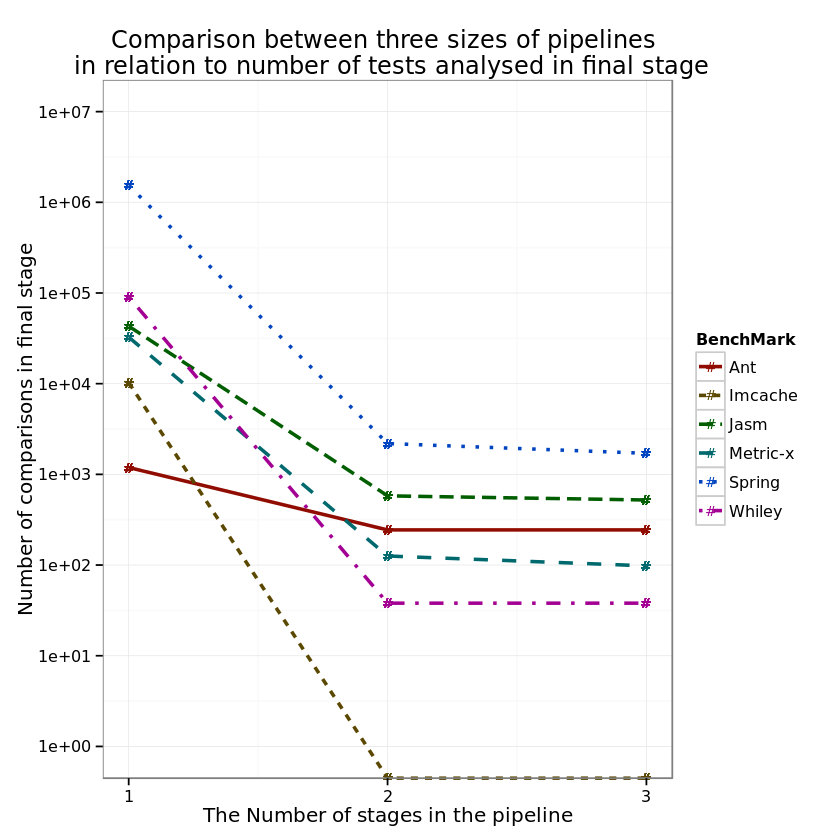
\includegraphics[height=10cm, width = 14.5cm]{Pipeline.png}
\end{center}
\caption{A figure showing the effect that the different pipeline lengths have on the number of comparisons during the final stage (Most computationally heavy). It is noted that the number of comparisons for a pipeline of length can be infered from the number of comparisons performed in the first pipeline stage in a pipeline of length two.}
\label{fig:pipelinegraph}
\end{figure}

\subsection{Discussion}

Inspecting Figure \ref{fig:pipelinegraph}, it becomes clear that the pipeline length decreases the comparisons in the final stage, but the length does not scale in every benchmark. This is shown by every two or three stage pipeline being a significant improvement on a single stage. However the majority of the benchmark's perform better with a two stage over a three. These results imply that the majority of the benchmarks were spending more time on the second stage than they were saving from the reduced number of comparisons in the third stage. There is one scenario proposed which would cause this. This scenario is that there may be little difference between the outcome from the second and third stages. Figure \ref{fig:stagesinpipeline} shows that this is what is happening. The figure shows that at the `output' on the x axis, the majority of benchmarks are under 100 comparisons. This means the third stage would only be performing a small number of comparisons. We would expect that the tests identified at that point are highly redundant and the third stage would not identify many more tests. To understand how this affects the outcome, we can inspect Figure \ref{fig:pipelinecomp}. The first stage in the pipelines has a large reduction in the number of comparisons between the input and output. Inspecting the pipeline of length three, the second stage reduces the number of test pairs by a limited amount. This creates a situation where the number of identified redundant test cases has little change from stage two to three while still performing the extra comparisons. Taking this discussion into account, as well as the factor that a pipeline of length one could take days to complete. This leads us to accept the first hypothesis, that increasing the pipeline length decreases the time taken and number of comparisons in the final stage. The optimal length of the pipeline may not be the same in every benchmark.

The change in the number of redundant tests identified is the other result to examine. The pipeline length of two had no significant difference to a length of three. If there was a change between the pipeline outputs while using the same final stage settings, this could imply two things. Firstly, the second pipeline stage is more specific than the third. Since both pipelines of length two and three share the same settings in final stage, for the pipeline of length three, the second stage may be identifying a higher similarity than the final stage. This would cause a different output between the two lengths. Secondly, there is a bug in the code.

\begin{figure}[h]
\centering
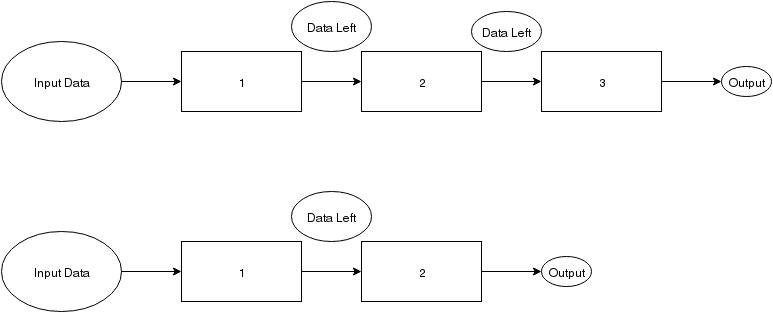
\includegraphics[width=\textwidth,height=8cm]{PipelineComp.png}
\caption{The circle size represents the data that is left in the pipeline. The figure shows that the difference that is between a two stage pipeline and a three stage only has limited room for a reduction in test cases identified. This shows the time taken to execute the extra stage costs more than it saves.}
\label{fig:pipelinecomp}
\end{figure}

\section{Experiment \rom{2} - K Depth Comparison}
\label{kdepthcomp}
\subsection{Motivation}
One of the abilities of the tool is to trace a call tree to the depth of K. This experiment is to determine the impact that altering the depth of K has on the overall cost. 

Increasing the depth of the call tree leads to an increase in the amount of data that is analysed, intuitively making it more difficult for test cases to be the same. We expect a reduction in the number of tests identified to be reflect this. The extra analysis performed implies an increase in the time taken. This time taken should not be substantial and we expect that the precision increase is worth the performance decrease. Hypothesis 2 reflects this.

\begin{hyp}
The precision improvement from increasing K Depth outweighs the performance decrease.
\end{hyp}

\subsection{Settings}
There are three K depth's explored, one, two and three respectively. It is important to note that a Wilcoxon signed-rank test was not performed as it is a two-sample test. We considered other significant tests to perform the test for three samples, however we felt the graphs were enough to convey the results.


\subsection{Results}
Ant, Whiley and Spring appear to be the most responsive to the depth of K as shown in Figure \ref{fig:kdepthgraph} albeit by a limited amount. The use of a log scale should be taken into account when looking at the graph as it may make the changes appear less notable. Figure \ref{fig:kdepthtime} shows the differences in time taken. Overall, for every benchmark there wasn't a large amount of change however it shows that as the K depth increases, the time taken increases. 

\begin{figure}[h]
\begin{center}
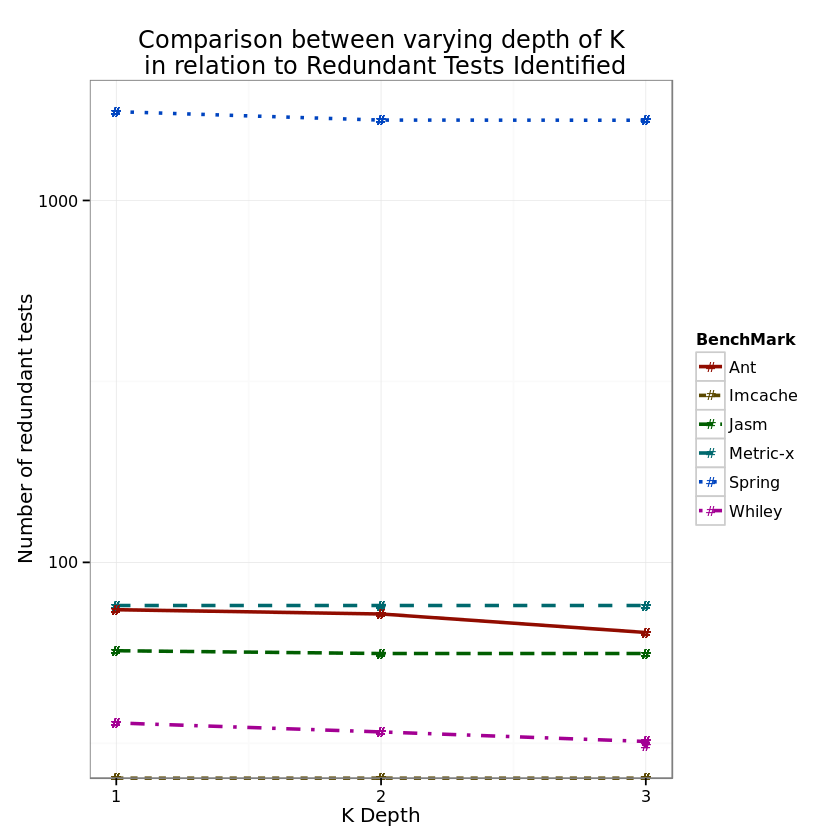
\includegraphics[height=10cm, width = 14.5cm]{KDepth.png}
\end{center}
\caption{A figure showing the effect that a change in the depth of the call tree has on the number of redundant tests are identified.}
\label{fig:kdepthgraph}
\end{figure}

\begin{figure}[h]
\centering
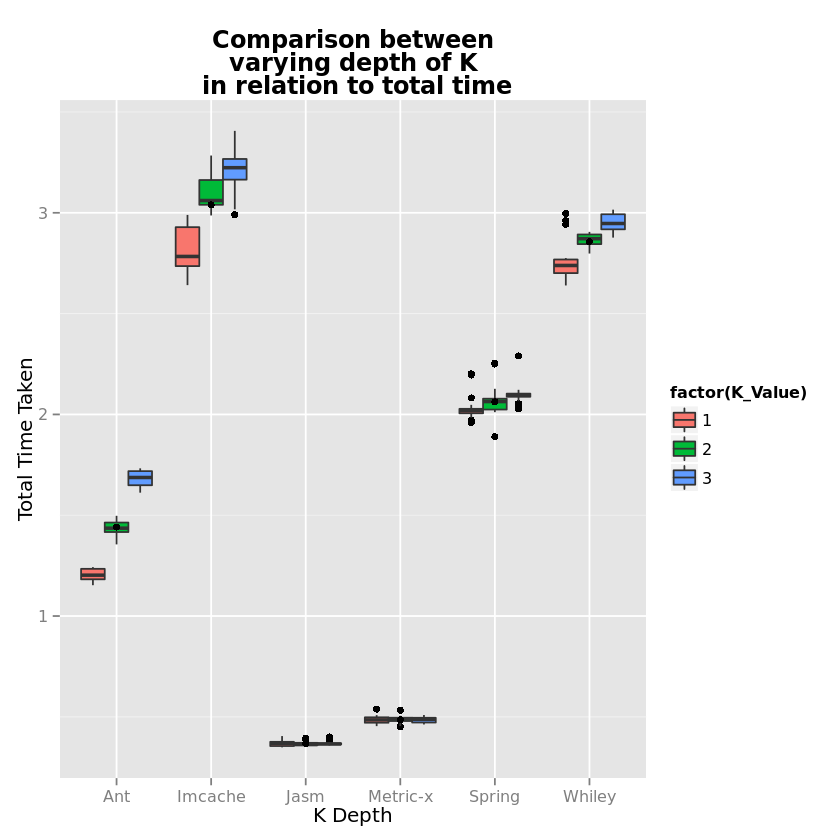
\includegraphics[width=\textwidth,height=13cm]{KDepthTime.png}
\caption{A figure showing the relationship that using a different K Depth has on the total time taken to analyse the data.}
\label{fig:kdepthtime}
\end{figure}

\subsection{Discussion}
There are two main take away points from the results. Firstly, it implies that when no other settings such as weighting or parameters are used, the depth has limited effect on the number of redundant test cases identified. Secondly, the number of comparisons that were output from the first pipeline stage may cause there to be a limited differentiation. When the first pipeline stage outputs a limited number of pairs, the final number of redundant tests identified would be similar regardless of the K depth specified. This situation is similar to the one discussed in Section \ref{sec:pipelineEva} and occurs in Whiley, Metric-x, Imcache and Jasm. The results from this experiment and Experiment \rom{1} indicate that by using a ``unique method call" filter and analysing a subset of the data, the tool is able to remove a large majority of the non-redundant tests. We can examine Figure \ref{fig:stagesinpipeline} to confirm this. Inspecting the figure, it shows that the heuristic pipeline removes a large portion of the comparisons between stage one and two. However, we need to inspect the number of output. The difference between pipeline stage two and the output is a limited amount. This shows that the heavy computational analysis stage only removes a small set of extra tests, this implies that the heuristic has a good accuracy of identifying redundant tests.
\begin{figure}[h]
\centering
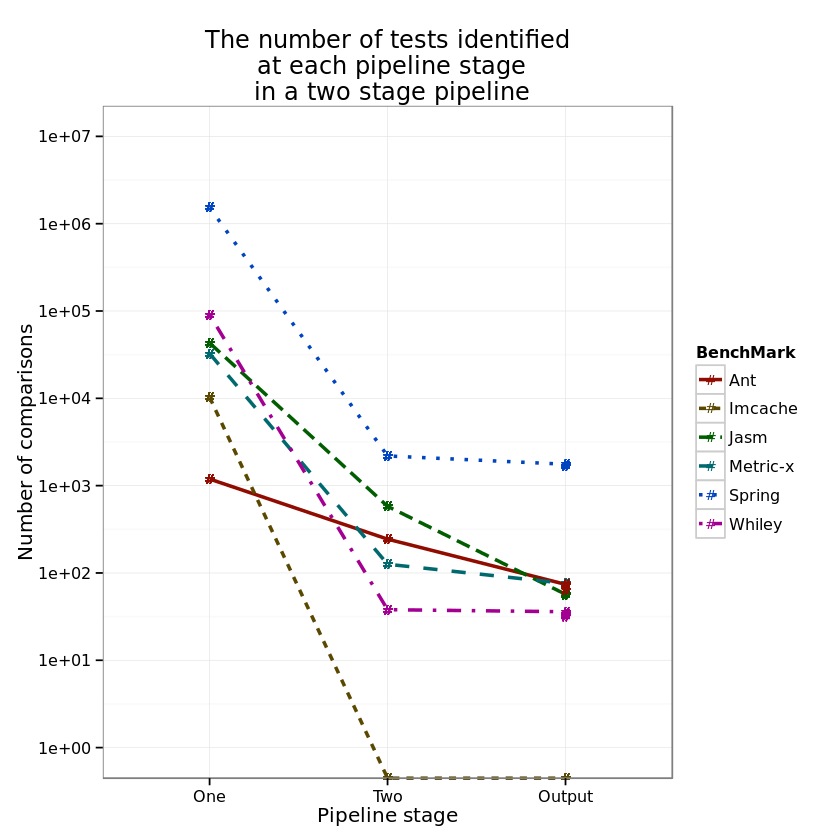
\includegraphics[width=\textwidth,height=11cm]{stagesinpipeline.png}
\caption{A figure showing the the number of comparisons that each stage performs. The pipeline contains two stages and is from Experiment \rom{1}. The graph shows the first stage is able to reduce a large number of the comparisons that the subsequent stage has to perform. \textbf{Note} this differs from Figure \ref{fig:pipelinegraph} as this looks at the number of comparisons in each stage. Figure \ref{fig:pipelinegraph} examines the comparisons performed in the final stage with varying pipeline lengths.}
\label{fig:stagesinpipeline}
\end{figure}

There is small change in the number of redundant tests identified, however we need to also examine the change in time taken. Increasing the depth of K has varying effect's on the time taken to analyse a benchmarks trace data. Figure \ref{fig:kdepthtime} shows the differences. It shows that Ant, Imcache and Whiley have larger differences than the rest, however in the perspective of time these equate to around half a minute difference. Although increasing the depth has an smaller effect than expected on precision, the impact on time taken isn't substantial. Taking this into account, I can accept the hypothesis with the results implying that for some projects the calling context does not have to be particularly deep. 

\section{Experiment \rom{3} - Parameter Comparison}
\label{sec:param}

\subsection{Motivation}
Parameters show the different contexts that a method was being called in. Retrieving this information gives us more confidence in determining whether two tests are redundant. The experiment explores the impact on performance and precision.

We need to take into account two factors when discussing the impact of parameters on the time taken. Firstly, it is intuitive that analysing the extra data generated increases the time. The amount of increase is interesting, parameters only add extra computation when the method execution of the given K is exactly the same. For example, if the test execution $A \rightarrow  B \rightarrow  C$ is compared to $A \rightarrow  B \rightarrow  F$ then the parameter won't be taken into account. Therefore parameters have limited effect on the time taken. 

The amount of time that the VM spends garbage collecting would also increase the time taken. Due to the increased amount of information in memory, the garbage collection process will have to execute more frequently for the analysis to continue to run. This would cause non-deterministic attributes to become more wide spread. Hypothesis 3 and 4 reflect this. These state that parameters increase the precision and the total time taken in comparison to the pipeline of length two in Experiment \rom{1}.

\begin{hyp}
Utilising parameters increases the time taken in comparison to a two stage pipeline.
\end{hyp}

\begin{hyp}
Utilising parameters increases the precision in comparison to a two stage pipeline.
\end{hyp}

\subsection{Settings}
The use of parameters is compared directly to the pipeline of length two used in Experiment \rom{1}.

\subsection{Results}
 Table \ref{parametersig} shows the comparison information between parameters and no parameters. It shows that there was a significant increase for every benchmark in regard to time taken. The table also shows that every benchmark had a significant decrease for the number of redundant test cases identified. This is not the case in Imcache due to it having zero redundant test cases identified in both. Examining Appendix \ref{fig:paramtime} -- Ant, Imcache, Jasm and Spring appear to affected by an increased variance between executions.
 
\begin{table}[h]
\centering
\begin{tabular}{|l|l|l|}
\hline
{\bf }          & {\bf Total Time} & {\bf Redundant Tests Identified} \\ \hline
{\bf Whiley}    & +                & -                           \\ \hline
{\bf Jasm}      & +               & -                          \\ \hline
{\bf Ant}       & +                & -                           \\ \hline
{\bf Spring}    & +                & -                           \\ \hline
{\bf Imcache}   & +                & =                           \\ \hline
{\bf Metrics-x} & +                & -                           \\ \hline
\end{tabular}
\caption{A table showing the significant relationship between the use of parameters and no parameters for each benchmark}
\label{parametersig}
\end{table}

\begin{figure}[h]
\begin{center}
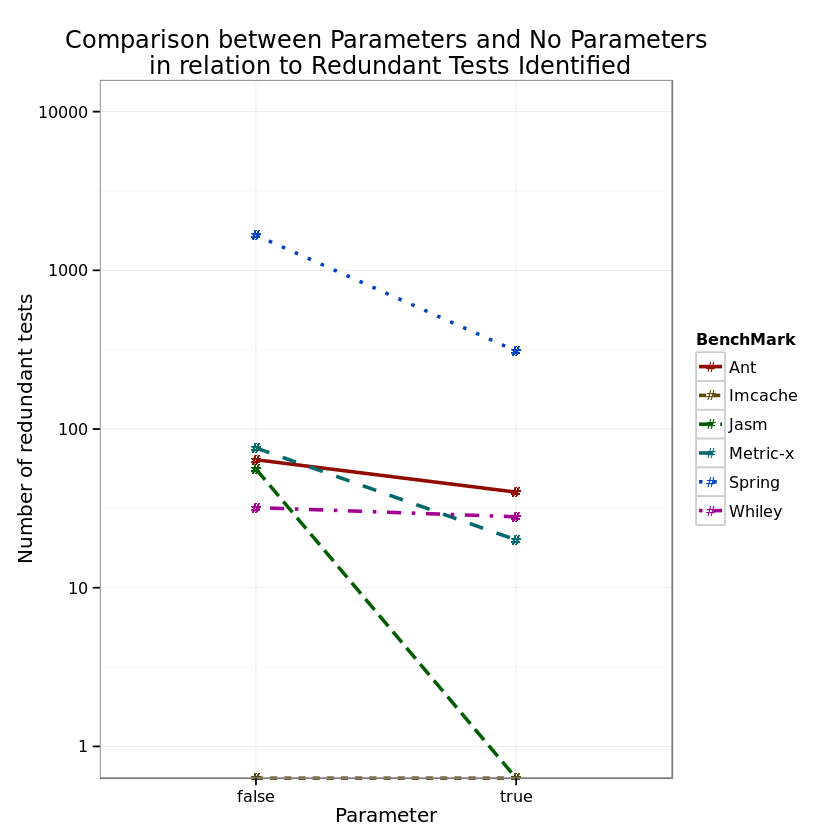
\includegraphics[height=10cm, width = 14.5cm]{Parameters.png}
\end{center}
\caption{A figure showing the effect that using parameters has on the number of redundant tests are identified.}
\label{fig:paramgraph}
\end{figure}


\subsection{Discussion}
The significant Table \ref{fig:paramgraph} matches what is expected. For every benchmark, using parameters significantly increases the time taken. Examining Appendix \ref{fig:paramtime} shows how the benchmarks react with more detail. The most interesting would be Jasm. Without parameters, it analyses the data in less than one minute, with parameters, it takes just under five minutes. This may be indicative of the results discussed in Section \ref{kdepthcomp}. The section discussed how increasing the K depth had little impact on the final outcome. Taking this into account, the call trees were matching the majority of the time and led to parameter information being examined more often, sequentially causing an increase in time taken. A factor that may have an accumulative effect are the setup and tear down methods. If these methods are a large majority of the method calls, and match each other for the K depth, this would further increase the time taken. This allows us to accept hypothesis 3 that parameters increase the time taken.

Looking at Figure \ref{fig:paramgraph}, it confirms that every benchmark reacted with a substantial decrease in redundant tests identified. Whiley was the least affected. This reiterates the discussion in Section \ref{kdepthcomp} that K depth is not enough of a factor to identify redundant test cases. To determine the precision improvement, we need to analysis the number of false positives identifiede.  At this stage, there is not enough information to perform this analysis. Hypothesis 4 will be revisited in Section \ref{addAnaly} where a stronger conclusion can be made.

\section{Experiment \rom{4} - Weighting Comparison}
\label{sec:weight}

\subsection{Motivation}
Utilising weighting is an attempt to remove any false positive tests identified. The experiment attempts to identify if applying the weighting technique has potential to remove these false positives. It also provides information concerning the impact on performance.

As discussed in Section \ref{C:related}, much of the related work encountered difficulties with test cases sharing setup and teardown method calls. This results in a high false positive rate. Intuitively, this makes sense when the test cases are small in comparison to the setup and teardown methods where these methods represent a large majority of the trace data. The approach of removing a part of the most executed method calls meant that the amount of data per test case decreases. This should reflect onto the results by showing a decrease in the time taken, as per hypothesis 7. The effect the weighting technique has on the number of redundant test cases should be dependent on the benchmark. This is because removing the most common tests should imply a decreased false-positive rate, but also may increase the number of actual redundant tests picked up. Hypothesis 6 reflects our interest in the precision difference.

\begin{hyp}
Weighting decreases the number of false positives compared to a standard two stage pipeline
\end{hyp}

\begin{hyp}
Weighting decreases the time taken compared to a standard two stage pipeline
\end{hyp}

\subsection{Settings}
The use of weighting is compared directly to the pipeline of length two settings in Experiment \rom{1}.


\subsection{Results}
There are a mixture of results concerning the total time taken. We see this in Table \ref{weightingsig} -- Whiley, Ant and Imcache had a significant increase in the time taken to analyse. Jasm, Spring and Metric-x had a significant decrease in the time taken to analyse. The majority -- Whiley, Ant, Jasm and Metrics-x had a significant decrease in the number of redundant tests identified. Spring was the only benchmark where weighting significantly increased the number of redundant tests identified.

\begin{table}[h]
\centering


\begin{tabular}{|l|l|l|}
\hline
{\bf }          & {\bf Total Time} & {\bf Redundant Tests Identified} \\ \hline
{\bf Whiley}    & +                & -                           \\ \hline
{\bf Jasm}      & -                & -                           \\ \hline
{\bf Ant}       & +                & -                           \\ \hline
{\bf Spring}    & -                & +                           \\ \hline
{\bf Imcache}   & +                & =                           \\ \hline
{\bf Metrics-x} & -                & -                           \\ \hline
\end{tabular}
\caption{A table showing the significant relationship between the use of weighting and no weighting for each benchmark}
\label{weightingsig}
\end{table}


\begin{figure}[h]
\begin{center}
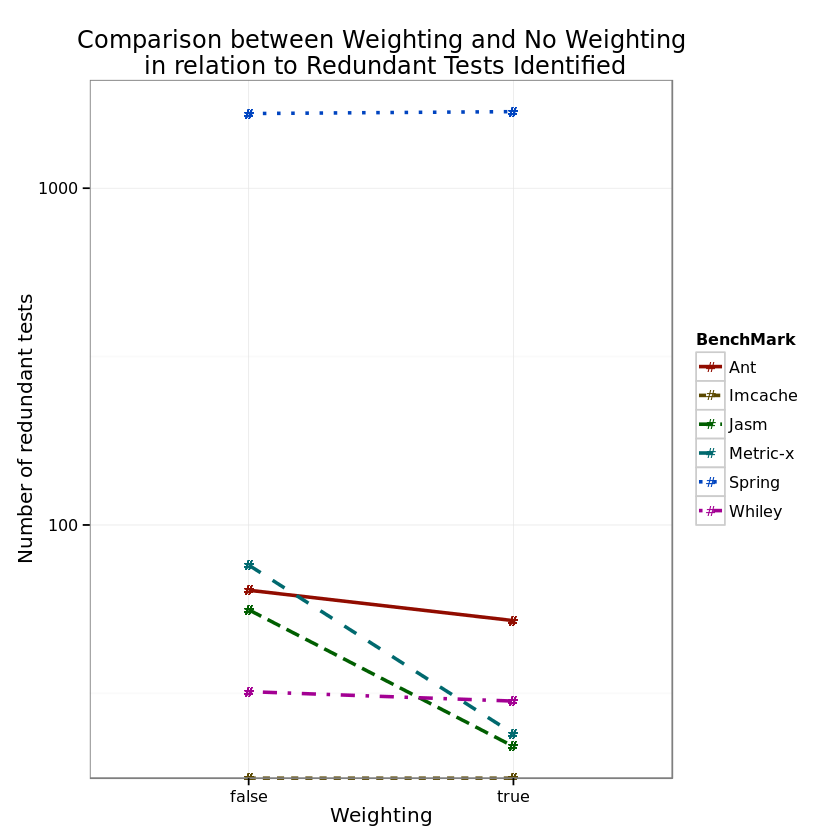
\includegraphics[height=10cm, width = 14.5cm]{Weighting.png}
\end{center}
\caption{A figure showing the effect that using weighting has on the number of redundant tests are identified.}
\label{fig:weightgraph}
\end{figure}

\subsection{Discussion}
A reduction in the false positive rate was the weighting techniques primary goal. Spring was the only benchmark that had a significant increase in the number of redundant test cases identified. The other benchmarks had a significant decrease. At first, this makes it appear that by using weighting it may solve some of the issues Maurer et al  \cite{koochakzadeh2009test} and Robinson et al. \cite{li2008static} identified. At this stage, there is not enough information to perform the analysis. Hypothesis 6 will be revisited in Section \ref{addAnaly} where a stronger conclusion can be made.

Table \ref{weightingsig} shows a mixture of results in regard to the total time taken. Two out of the three benchmarks that had a significant increase in the total time were small benchmarks -- Whiley, Ant, Imcache. This may imply that the size of the benchmark has some relation to the effect of weighting on the time taken. One reason is that the tool calculates weighting once per test case per analysis stage. The weighting calculation has a linear relation with the number of test cases. In comparison, the tool compares every test case to every other. This is a squared relation with the number of test cases. The less test cases there are, the closer the linear relation is to the squared and the more impact the linear weight calculation has on the time taken. This may explain a relation between size and time taken. Appendix \ref{fig:weighttime} shows the overview of the impact on the time taken . The figure shows there was no general impact from using weighting on the benchmarks. Taking the discussion into account, it allows us to invalidate hypothesis 7 and that weighting does not affect time taken.

\section{Additional Analysis}
\label{addAnaly}
It is not enough for the tool to identify tests. We need to examine these tests and verify that the tests identified are truly redundant and not false positives. To achieve this, we manually classified the identified tests into types of redundancy. The types of redundancy are where there are only slight differences and the names given to the types are indicative of the main differences between the tests. The test data was taken directly from the experiments discussed throughout the chapter including data from a pipeline using both parameters and weighting. As the classification was a lengthy process, only Whiley and Metric-x had their output tests classified. This section will continue the discussion from Sections \ref{sec:param} and \ref{sec:weight} and conclude the hypothesises.

\subsection{Parameters}

In Section \ref{sec:param}, we discussed that parameters caused a decrease in the number of tests identified. We need to inspect the types of tests identified to conclude hypothesis 4. The hypothesis states that parameters increases the precision in comparison to a two stage pipeline. Inspecting Table \ref{whileycoding} and \ref{metriccoding} gives insight into the types of tests identified. The Whiley benchmark coding shows that parameters remove the limited redundant tests as well as different array values. The Metric-x coding demonstrates a reduction in the number of the different parameter value tests identified substantially, from 52 to 8. These coding show that we are able to reduce the number of redundancies identified without losing any fully redundant tests. Taking these coding tables into account, it allows us to accept hypothesis 4 that parameters increase the precision.

\subsection{Weighting}

Revisiting hypothesis 6, it states that weighting decreases the number of false positives compared to a standard two stage pipeline. To confirm this, examining Table \ref{whileycoding} and \ref{metriccoding} will give insight into the effect of weighting. Comparing the two columns for the Whiley coding, Pipeline 2 and Weighting, the only difference is the removal of the two limited redundancy test cases that were picked up by Pipeline 2. This shows the weighting technique is able to reduce the impact that the similar set up and tear down methods have on the analysis. By removing the method executions that were common, this led to a decrease in the number of false positive tests identified. The Metric-x coding is a similar result. The weighting technique reduces the number of parameter value redundancies identified as well as the limited redundancies, but does not completely remove them. This is interesting and implies that the number of setup and tear down methods that remained in the data analysed was still a large part of the data. We are able to accept hypothesis 6, although work remains to improve the weighting method to remove redundant tests completely.

\subsection{Further Discussion}

Neither weighting or parameters were able to fully remove the tests with limited redundancy in Table \ref{metriccoding}. The table suggests that the combination of parameters and weighting may have some appeal by removing all eight limited redundancy tests. At the same time, the similar tests are also removed which is a negative outcome. This suggests that the combination may have some applicability to other benchmarks and may warrant future experiments on it.

\begin{table}[h]
\centering

\begin{tabular}{|l|l|l|l|l|}
\hline
                          & \multicolumn{4}{c|}{{\bf Whiley}}                                                             \\ \hline
{\bf Types of redundancy} & \multicolumn{1}{c|}{{\bf Pipeline 2}} & {\bf Weighting} & {\bf Parameters} & {\bf Parameters and Weighting} \\ \hline
Different Equation Value  & 6                                     & 6               & 6                & 6                \\ \hline
Different Equation Sign   & 8                                     & 8               & 8                & 8                \\ \hline
Different Array Values    & 2                                     & 2               & 0                & 0                \\ \hline
Same                      & 10                                    & 10              & 10               & 10               \\ \hline
Limited Redundancy        & 2                                     & 0               & 0                & 0                \\ \hline
Rearranged Equation       & 2                                     & 2               & 2                & 2                \\ \hline
Extra if statement        & 2                                     & 2               & 2                & 2                \\ \hline
                          &                                       &                 &                  &                  \\ \hline
{\bf Total}               & 32                                    & 30              & 28               & 28               \\ \hline
\end{tabular}
\caption{A table displaying a list of coding's for the Whiley Benchmark for four of the different techniques used. The tests identified have been coded under a type of redundancy. These types of redundancies allow us to see how many false-positives were identified as being redundant. }
\label{whileycoding}
\end{table}


\begin{table}[]
\centering
\begin{tabular}{|l|l|l|l|l|}
\hline
                             & \multicolumn{4}{c|}{\textbf{Metric-X}}                                                              \\ \hline
\textbf{Types of redundancy} & \textbf{Pipeline 2} & \textbf{Weighting} & \textbf{Parameters} & \textbf{Parameters  And Weighting} \\ \hline
Different Parameter Value    & 52                  & 10                 & 8                   & 4                                  \\ \hline
Different Object Type        & 6                   & 2                  & 2                   & 0                                  \\ \hline
Different Array Values       & 8                   & 6                  & 4                   & 6                                  \\ \hline
Similar                      & 2                   & 2                  & 0                   & 0                                  \\ \hline
Limited Redundancy           & 8                   & 4                  & 6                   & 0                                  \\ \hline
\textbf{}                    &                     &                    &                     &                                    \\ \hline
\textbf{Total}               & 76                  & 24                 & 20                  & 10                                 \\ \hline
\end{tabular}
\caption{A table displaying a list of coding's for the Whiley Benchmark for four of the different techniques used. The tests identified have been coded under a type of redundancy. These types of redundancies allow us to see how many false-positives were identified as being redundant.}
\label{metriccoding}
\end{table}

\section{Limitations}

\begin{itemize}

\item A major limitation to the study was the amount of RAM used. For the Whiley and Ant benchmarks, the tool had high RAM usage when storing the parameter data and call tree information. This limited the amount of tests that it was able to retrieve. The experiments may not fully represent the total redundancy in these two benchmarks.

\item Some of the benchmarks that we chose contain multiple unit tests within one test case. The tool described throughout this report would not be able to pick up when a test case subsumes another. The tool only looks at the method call information, as such gains no new information by identifying method call subsumed tests. It is then difficult gauge this type of redundancy within the test suites.

\item Some benchmarks performed better with a two stage pipeline in comparison to a three stage, and vice versa. A range of different settings were tested to identify close to optimal settings for the second stage. However, this does not mean that the settings chosen were optimal and may have skewed the data slightly.

\item The tool applies the weighting technique once per stage where required. Performing the calculation once per stage is adds unnecessary calculations. This does not affect the experiments as weighting is ever only executed once per pipeline.
\end{itemize}
